\documentclass[sigplan,10pt,review]{acmart}\settopmatter{printfolios=true,printccs=false,printacmref=false}
\usepackage[normalem]{ulem} % double underline
\usepackage{fontspec}
\setmonofont{Cabin}
\setmonofont{Comfortaa}
\setmonofont{Latin Modern Mono Light 10 Bold}
% \setmonofont{FreeMono Bold}
\usepackage{listings}
\definecolor{dkblue}{rgb}{0,0.1,0.5} 
\definecolor{lightblue}{rgb}{0,0.5,0.5} 
\definecolor{dkgreen}{rgb}{0,0.4,0} 
\definecolor{dk2green}{rgb}{0.4,0,0} 
\definecolor{dkviolet}{rgb}{0.6,0,0.8}
%\renewcommand*{\ttdefault}{lmss}
\def\lstlanguagefiles{defManSSR.tex,lstlang2.sty}
\lstset{language=SSR, breaklines=false} %flexiblecolumns=false, 
\lstset{moredelim=[is][\uline]{|*}{*|}}
\lstset{moredelim=[is][\uwave]{/+}{+/}}
\lstset{moredelim=[is][\uline]{/*}{*/}}
\lstset{moredelim=[is][\color{dkblue}]{|+}{+|}}

\usepackage[english]{babel}
\usepackage{menukeys}
\newcommand{\derive}[1]{\keys{#1}}

\usepackage{draftwatermark}
\SetWatermarkText{Draft}

%\usepackage{minted}
%\newminted{coq}{fontsize=\footnotesize,escapeinside=\#\#}
 
%% Conference information
%% Supplied to authors by publisher for camera-ready submission;
%% use defaults for review submission.
\acmConference[PL'18]{ACM SIGPLAN Conference on Programming Languages}{January 14--15, 2019}{Lisbon, Protugal}
\acmYear{2019}
\acmISBN{} % \acmISBN{978-x-xxxx-xxxx-x/YY/MM}
\acmDOI{} % \acmDOI{10.1145/nnnnnnn.nnnnnnn}
\startPage{1}

%% Copyright information
%% Supplied to authors (based on authors' rights management selection;
%% see authors.acm.org) by publisher for camera-ready submission;
%% use 'none' for review submission.
\setcopyright{none}
%\setcopyright{acmcopyright}
%\setcopyright{acmlicensed}
%\setcopyright{rightsretained}
%\copyrightyear{2018}           %% If different from \acmYear

%% Bibliography style
\bibliographystyle{ACM-Reference-Format}


\usepackage{booktabs}
\usepackage{subcaption}

\begin{document}

\title{Deriving proved equality tests in Coq-elpi}
%\titlenote{with title note}
\subtitle{Stronger induction principles for containers in Coq}
%\subtitlenote{with subtitle note}

\author{Enrico Tassi}
\orcid{nnnn-nnnn-nnnn-nnnn}             %% \orcid is optional
\affiliation{
  \institution{Universit\'e c\^ote d'Azur - Inria}
}
\email{Enrico.Tassi@inria.fr}          %% \email is recommended



%% Abstract
%% Note: \begin{abstract}...\end{abstract} environment must come
%% before \maketitle command
\begin{abstract}
We describe a procedure to derive equality tests and their correctness
proofs from inductive type declarations.  Programs and proofs
are derived compositionally, reusing code and proofs derived
previously.  

The key steps are two. First, we
design stronger induction principles for data types defined
using parametric containers. Second, we
develop a technique to work around the modularity limitations
imposed by the purely syntactic termination check Coq performs
on recursive proofs. 
The unary parametricity translation of inductive data types
turns out to be the key to both steps.

Last but nor least, we provide an implementation of the procedure
for the Coq proof assistant based on the Elpi extension language.
\end{abstract}


%% 2012 ACM Computing Classification System (CSS) concepts
%% Generate at 'http://dl.acm.org/ccs/ccs.cfm'.
\begin{CCSXML}
<ccs2012>
<concept>
<concept_id>10011007.10011006.10011008</concept_id>
<concept_desc>Software and its engineering~General programming languages</concept_desc>
<concept_significance>500</concept_significance>
</concept>
<concept>
<concept_id>10003456.10003457.10003521.10003525</concept_id>
<concept_desc>Social and professional topics~History of programming languages</concept_desc>
<concept_significance>300</concept_significance>
</concept>
</ccs2012>
\end{CCSXML}

\ccsdesc[500]{Software and its engineering~General programming languages}
\ccsdesc[300]{Social and professional topics~History of programming languages}
%% End of generated code


%% Keywords
%% comma separated list
\keywords{Coq, Containers, Induction, Equality test, Parametricity
translation}  %% \keywords are mandatory in final camera-ready submission


%% \maketitle
%% Note: \maketitle command must come after title commands, author
%% commands, abstract environment, Computing Classification System
%% environment and commands, and keywords command.
\maketitle

\section{Introduction}

Modern typed programming languages come with the ability of generating
boilerplate code automatically. Typically when a data type is declared
a substantial amount of code is made available to the programmer at
little cost, code such as a comparison function, a printing function,
generic visitors etc.  The \lstinline+derive+ directive of Haskell or the
\lstinline+ppx_deriving+ OCaml preprocessor provide these features for the
respective programming language.

The situation is less than ideal in the Coq proof assistant.  It is
capable of synthesizing the recursor of a datatype, that,
following the Curry-Howard isomorphism, implements the induction
principle associated to that datatype. It supports all datatypes,
containers such as lists included, but generates a quite disappointing
principle when a datatype \emph{uses} a container.

For example, let's take the data type rose tree, where \lstinline+U+
stands for a universe (such as \lstinline+Prop+ or \lstinline+Type+):

\begin{minipage}{\textwidth}\begin{lstlisting}
Inductive rtree A : U :=
| Leaf (a : A)
| Node (l : list (rtree A)).
\end{lstlisting}\end{minipage}

\noindent
Its associated induction principle is the following one:

\begin{minipage}{\textwidth}\begin{lstlisting}[numbers=left]
Lemma |+rtree_ind+| : forall A (P : rtree A -> U),
    (forall a : A, P (Leaf A a)) ->
    (forall l : list (rtree A), P (Node A l)) ->
  forall r : rtree A, P r.
\end{lstlisting}\end{minipage}

Remark that the recursive step, line 3, lacks any induction hypotheses
on (the elements of) \lstinline+l+ while one would expect
\lstinline+P+ to hold on each and every subtree.  Coq provides
an additional facility to synthesize equality tests and their proofs
called \lstinline+Scheme Equality+, but containers are not supported.
The \lstinline+decide equality+ tactic can be manually iterated in
order to generate a (proof) term implementing an equality tests for
the type above, but this requires human intervention and also
generates large terms since it inlines both the equality tests and the 
correctness proofs for all the containers used.

The state of affairs is particularly unfortunate because
the need for the automatic generation of boilerplate
code in the Coq ecosystem is higher than ever.
Modern formal libraries structure their contents in a
hierarchy of interfaces and some machinery such as type classes or
canonical structures are used to link the abstract library to the
concrete data the user is working on.  For example first interface one
is required to implement in order to use the theorems in Mathematical
Components library on a type \lstinline+T+ is the \lstinline+eqType+
one, that requires a correct equality test on \lstinline+T+.

% We see two reasons behind the current state of affairs.
% On one hand the data types one can declare in Coq are very rich,
% making program synthesis hard and proof synthesis even harder.
% On the other hand high level tools
% for meta programming Coq only recently started to appear.
% The derivations described above are coded in OCaml, eg manipulating De
% Bruijn indexes. Experimenting on a derivation is quite expensive.

In this paper we use the framework for meta programming based on Elpi
developed by the author and we focus on the derivation of an instance
of the
\lstinline+eqType+ structure for a given data type.
The aim is to provide a practical tool that is both automatic and
avoids duplication and inlining whenever possible.

It turns out that generation of equality tests is relatively easy,
while their proofs are hard, for two reasons. The first problem is that 
the standard induction principles generated by Coq, as depicted
before, are too weak. In order to fix them one needs quite some extra
boilerplate, such as the derivation of the unary parametricity
translation of the data types involved.
The second one is that termination checking
is purely syntactic in Coq. Rephrased along the Curry-Howard
isomorphism this means that in order to check that the induction
hypothesis is applied to a smaller term, Coq may need to unfold all
terms involved in the proof. This, in practice, it forces all proof to
be transparent breaking modularity: a statement is no more contract,
changing its proof script may impact users.

In this paper we describe a derivation procedure for the
\lstinline+eqType+ structure where programs and proofs are both
derived compositionally, reusing code and proofs derived previously.
This procedure also confines the termination check issue,
allowing proofs to be mostly opaque.

More precisely the contributions of this paper are the following ones:
\begin{itemize}
\item A technique to confine the termination checking issue out of the
	main proofs. In this paper we apply it to the proof of equality
	tests, but it is applicable to all proofs by structural
	induction.

\item A modular and structured process to derive instances of the
	\lstinline+eqType+ structure and, en passant, stronger
	induction principles for inductive types defined using
	containers.

\item An actual implementation based on the Elpi extension language
	for the Coq proof assistant.
\end{itemize}

\noindent
Straight to the point, by installing the \lstinline+coq-elpi-derive+
package\footnote{See \url{https://github.com/LPCIC/coq-elpi} for the
installation instructions} 
one obtains the following definition, where \lstinline+reflect P b+
is a predicate stating the equivalence between a predicate
\lstinline+P+ and a boolean test \lstinline+f+.

\begin{minipage}{\textwidth}\begin{lstlisting}
Definition eq_axiom T f x :=
  forall y, reflect (x = y) (f x y).
\end{lstlisting}\end{minipage}

\noindent
Then by issuing the command \lstinline+Elpi derive rtree+ one gets
the following terms automatically synthesized out of the type
declaration for \lstinline+rtree+:

\begin{minipage}{\textwidth}\begin{lstlisting}
Definition |+rtree_eq+| :
  forall A, (A -> A -> bool) -> rtree A -> rtree A -> bool.

Lemma |+rtree_eq_OK+| : forall A (A_eq : A -> A -> bool),
    (forall a, eq_axiom A A_eq a) ->
  forall r, eq_axiom (rtree A) (rtree_eq A A_eq) r.
\end{lstlisting}\end{minipage}

\noindent
The former is a (transparent) equality test for \lstinline+rtree+.
The latter is a (opaque) proof of correctness for \lstinline+rtree_eq+
under the assumption that the equality test \lstinline+A_eq+ is correct.

The paper introduces the problem in
section~\ref{sec:problem} by describing the shape of an equality test
and of its correctness proof and explaining the modularity problem
that stems for the termination checker of Coq. It then
presents the main idea behind the
modular derivation procedure in section~\ref{sec:idea}.
Section~\ref{sec:code} describes all the bricks composing the
derivation, while section~\ref{sec:elpi} briefly describes the
implementation in Elpi.
% In this paper we systematically omit the
% \lstinline+Definition+ and \lstinline+Lemma+ keywords: terms are given
% a type with \lstinline+:+ and eventually a body with \lstinline+=+.


%%%%%%%%%%%%%%%%%%%%%%%%%%%%%%%%%%%%%%%%%%%%%%%%%%%%%%%%%%%%%%%%%%%%%%%%%%%%%
\section{The problem: equality tests proofs meet syntactic termination checking} %%%%%
\label{sec:problem}

Recursors, or induction principles, are not primitive notions in Coq.
The language provides constructors for fix point and pattern matching
that work on any inductive data the user can declare.

For example to test two lists \lstinline+l1+ and \lstinline+l2+ for
equality one first takes in input an equality test \lstinline+A_eq+
for the elements of type \lstinline+A+ and then performs the
recursion:

\begin{minipage}{\textwidth}\begin{lstlisting}[numbers=left]
Definition |+list_eq+| A (A_eq : A -> A -> bool) :=
  fix rec (l1 l2 : list A) {struct l1} : bool :=
    match l1, l2 with
    | nil, nil => true
    | x :: xs, y :: ys => A_eq x y && rec xs ys
    | _, _ => false
    end.
\end{lstlisting}\end{minipage}

\noindent
Coq accepts this definition because
the recursive call is on \lstinline+xs+ that is a syntactically
smaller, i.e. a sub term, of the input term \lstinline+l1+ (the
argument labelled as decreasing by the \lstinline+{struct l1}+
annotation).

Lets new define the equality test for the \lstinline+rtree+ data type
by reusing the equality test for lists:

\begin{minipage}{\textwidth}\begin{lstlisting}[numbers=left,firstnumber=8]
Definition |+rtree_eq+| B (B_eq : B -> B -> bool) :=
  fix rec (t1 t2 : rtree B) {struct t1} : bool :=
    match t1, t2 with
    | Leaf x, Leaf y => B_eq x y
    | Node l1, Node l2 =>
        list_eq (rtree B) rec l1 l2
    | _, _ => false
    end.
\end{lstlisting}\end{minipage}

\noindent
Note that \lstinline+list_eq+ is called passing as the \lstinline+A_eq+
argument the fixpoint \lstinline+rec+ itself (line 13). In order to
check that the latter definition is sound, Coq looks at the body of
\lstinline+list_eq+ to see weather its parameter \lstinline+A_eq+ is
applied to a term smaller than \lstinline+t1+. Since
\lstinline+l1+ is a subterm of \lstinline+t1+ and that \lstinline+x+
is a subterm of \lstinline+l1+, the recursive call (line 5) is legit.

This is pretty reasonable for programs. We want both \lstinline+list_eq+
and \lstinline+rtree_eq+ to compute, hence their body matters to us.
The fact that checking the termination of \lstinline+rtree_eq+ requires
inspecting the body of \lstinline+list_eq+ is not very annoying this
time.

On the contrary proof terms are typically hidden to the type checker once
they have been validated, for both performance and modularity reasons.
The desire is to make only the statement of theorems binding, and keep
the freedom to clean, refactor, simplify proofs without breaking
the rest of the formal development. 

For example, lets assume we proved that \lstinline+list_eq+ is
correct.

\begin{minipage}{\textwidth}\begin{lstlisting}[numbers=left]
Lemma |+list_eq_OK+| : forall A (A_eq : A -> A -> bool),
    (forall a, eq_axiom A A_eq a) ->
  forall l, eq_axiom A (list_eq A A_eq) l.
Proof. .. Qed.
\end{lstlisting}\end{minipage}

It seems desiable to use this lemma in order to prove the
correctness of \lstinline+rtree_eq+, since it calls
\lstinline+list_eq+.

Unfortunately the following proof is rejected if the body of
\lstinline+list_eq_OK+ is hidden to the type checker:

\begin{minipage}{\textwidth}\begin{lstlisting}[numbers=left,firstnumber=5]
Lemma |+rtree_eq_OK+| B B_eq (H_B_eq: forall b, eq_axiom B B_eq b) :
  forall t, eq_axiom (rtree B) (rtree_eq B B_eq) t
:= 
  fix IH (t1 t2 : rtree B) {struct t1} :=
  match t1, t2 with
  | Node l1, Node l2 =>
    .. list_eq_OK (rtree B) (tree_eq B B_eq) IH l1 l2 ..
  | Leaf b1, Leaf b2 => .. H_B_eq b1 b2 ..
  | .. => ..
  end.
\end{lstlisting}\end{minipage}

\noindent
We pass \lstinline+IH+, the induction hypothesis, as the
witness that \lstinline+(tree_eq B fb)+ is a correct equality test
(the argument at line 10). Without knowing how this argument is used
by \lstinline+list_eq_OK+ Coq rejects the term.

The issue seems unfixable without changing Coq in order to use a more
modular check for termination, for example based on sized
types\cite{sacchini:pastel-00622429}.
We propose a less ambitious but more practical approach here, that
consists in putting the transparent terms that the termination checker
is going to inspect outside of the main proof bodies so that they can be 
kept opaque.

The intuition is to reify the property the termination checker wants
to enforce. It can be phrased as ``x is a subterm of t and has the same
type''. More in general we model ``x is a subterm of t with property
P`` and ``P`` is going to be ``beign of the same type`` for subterms
of ``t`` that are of the same type, while ``P`` will be an arbitrary
property for terms of an arbitrary type such as the elements of
a list.

This relation is naturally expressed by the unary parametricity
translation of types~\cite{Wadler:1989:TF:99370.99404}.
Thanks to the work of Keller and
Lasson~\cite{keller:hal-00730913} we have this translation for Coq.


%%%%%%%%%%%%%%%%%%%%%%%%%%%%%%%%%%%%%%%%%%%%%%%%%%%%%%%%%%%%%%%%%%%%%%%%%%%%%
\section{The idea: separating terms and types via the unary parametricity translation}
\label{sec:idea}

Given an inductive type \lstinline+T+ we systematically name \lstinline+is_T+
an inductive predicate describing the type of the inhabitants of
\lstinline+T+. This is the one for natural numbers:

\begin{minipage}{\textwidth}\begin{lstlisting}
Inductive is_nat : nat -> U :=
| is_O : is_nat 0
| is_S n (pn : is_nat n) : is_nat (S n).
\end{lstlisting}\end{minipage}

\noindent
The one for a container such as \lstinline+list+ is more interesting:

\begin{minipage}{\textwidth}\begin{lstlisting}
Inductive is_list A (PA : A -> U) : list A -> U :=
| is_nil : is_list A PA nil
| is_cons a (pa : PA a) l (pl : is_list A PA l) :
    is_list A PA (a :: l).
\end{lstlisting}\end{minipage}

\noindent
Remark that all the elements of the list validate \lstinline+PA+.

When a type \lstinline+T+ is defined in terms of another other type
\lstinline+C+, typically a container, the \lstinline+is_C+ predicate
shows up inside \lstinline+is_T+. For example:

\begin{minipage}{\textwidth}\begin{lstlisting}[numbers=left]
Inductive is_rtree A (PA : A -> U): rtree A -> U :=
| is_Leaf a (pa : PA a) : is_rtree A PA (Leaf A n)
| is_Node l (pl : is_list (rtree A) (is_rtree A PA) l) :
    is_rtree A PA (Node A l).
\end{lstlisting}\end{minipage}

\noindent
Note how line 3 expresses the fact that all elements in the list
\lstinline+l+ validate \lstinline+(is_rtree A PA)+.

Our intuition is that these predicates ``reify'' the notion of being
of a certain type, structurally. What we typically write \lstinline+(t : T)+
can now be also phrased as \lstinline+(is_T t)+ as one would do in a
framework other than type theory, such as a mono-sorted logic.

It turns out that the inductive predicate \lstinline+is_T+ corresponds
to the unary parametricity translation of the type \lstinline+T+.
Keller and Lasson~\cite{keller:hal-00730913} give us an
algorithm to synthesize these predicates automatically.

What we look for now is a way to synthesize
a reasoning principle for a term \lstinline+t+ when 
\lstinline+(is_T t)+ holds.

\subsection{Stronger induction principles for containers} %%%%%%%%%%%%%%%%%%%%%%%%%%%%%

Let's have a look at the standard induction principles of lists.

\begin{minipage}{\textwidth}\begin{lstlisting}
Lemma |+list_ind+| A (P : list A -> U) :
    P nil ->
    (forall a l, P l -> P (a :: l)) ->
  forall l : list A, P l.
\end{lstlisting}\end{minipage}

\noindent
This reasoning principle is purely parametric on \lstinline+A+, no
knowledge on any term of type \lstinline+A+ such as \lstinline+a+ is
ever available.

What we want to obtain is a more powerful principle that let as choose
some invariant for the subterms of type \lstinline+A+. The one we
synthesise is the following one, where the differences are underlined.

\begin{minipage}{\textwidth}\begin{lstlisting}[numbers=left]
Lemma |+list_induction+| A /*(PA: A -> U)*/ (P: list A -> U):
    P nil ->
    (forall a /*(pa : PA a)*/ l, P l -> P (a :: l)) ->
  forall l, /*is_list A PA l*/ -> P l.
\end{lstlisting}\end{minipage}

\noindent
Note the extra premise \lstinline+(is_list A PA l)+: The
implementation of this induction principle
goes by recusion on of the term of this type and finds
as an argument of the \lstinline+is_cons+ constructor
the proof evince \lstinline+(pa : PA a)+ it feeds to the second premise
(line 3). Our intuition is that all terms of type \lstinline+(list A)+
validate the property \lstinline+P+, while all terms of type
\lstinline+A+ validate the property \lstinline+PA+.

More in general to each type we attach a property. For parameters we
let the user choose (we take another parameter, \lstinline+PA+ here).
For the type being analyzed, \lstinline+list A+ here, we take the
usual induction predicate \lstinline+P+.
For terms of other types we use their unary parametricity translation.

Take for example the induction principle for \lstinline+rtree+.

\begin{minipage}{\textwidth}\begin{lstlisting}[numbers=left]
Lemma |+rtree_induction+| A PA (P : rtree A -> U) :
    (forall a, PA a -> P (Leaf A a)) ->
    (forall l, is_list (rtree A) P l -> P (Node A l)) ->
  forall t, is_rtree A PA t -> P t.
\end{lstlisting}\end{minipage}

\noindent
Line 3 uses \lstinline+is_list+ to attach a property to \lstinline+l+,
and given that \lstinline+l+ has type \lstinline+(list (rtree A))+
the property for the type parameter \lstinline+(rtree A)+ is
exactly \lstinline+P+.
Note that this induction principle give us access to \lstinline+P+, the
property one is proving, on the subtrees contained in \lstinline+l+.

\subsubsection{Synthesizing better induction principles} %%%%%%%%%%%%%%%%%

We postpone a detailed description of the synthesis to
section~\ref{sec:induction}, here we just sketch how to
build the type on the induction principle.

It turns out that the types of the constructors of
\lstinline+is_T+ give us a very good hint on the type
of the induction principle.

The type of the first premise, line 2 in the snippet above,
is exactly the type of the \lstinline+is_Leaf+ constructor
where \lstinline+(is_rtree A PA)+ is replaced by \lstinline+P+.
The same hold for the premise at line 3, that corresponds to
the type of \lstinline+is_Node+ provided the same replacement.

Our intuition is that the inductive predicate \lstinline+is_T+
provides the same information that typing provides. Induction
principles give \lstinline+P+ on (smaller) terms of the same type,
that would be terms for which \lstinline+is_T+ holds.

\subsection{Isolating the syntactic termination check} %%%%%%%%%%%
\label{sec:idea:transparent}

As one expects, it is possible to prove that \lstinline+is_T+
holds for terms of type \lstinline+T+.

\begin{minipage}{\textwidth}\begin{lstlisting}
Definition |+nat_is_nat+| : forall n : nat, is_nat n :=
  fix rec n : is_nat n :=
  match n as i return (is_nat i) with
  | 0 => is_O
  | S p => is_S p (rec p)
  end.
\end{lstlisting}\end{minipage}

\noindent
For containers we can prove this class of theorems
when the property on the
parameter is true on the entire type.

\begin{minipage}{\textwidth}\begin{lstlisting}
Definition |+list_is_list+| : forall A (PA : A -> U),
  (forall a, PA a) -> forall l, is_list A PA l.

Definition |+rtree_is_rtree+| : forall A (PA : A -> U),
  (forall a, PA a) -> forall t, is_rtree A PA t.
\end{lstlisting}\end{minipage}

\noindent
These facts are then to be used in order to satisfy the
premise of our induction principles. We can build correctness
proofs of equality tests in two steps.

For example, for natural numbers

\begin{minipage}{\textwidth}\begin{lstlisting}[numbers=left]
Lemma |+nat_eq_correct+| :
  forall n, is_nat n -> eq_axiom nat nat_eq n
:=
  nat_induction (eq_axiom nat nat_eq) PO PS.

Lemma |+nat_eq_OK+| n : eq_axiom nat nat_eq n :=
  nat_eq_correct n (nat_is_nat n).
\end{lstlisting}\end{minipage}

\noindent
Where \lstinline+PO+ and \lstinline+PS+ (line 2) stand for
the two proof terms corresponding to the base case and the inductive
step of the proof. We omit them because they play no role in the
current discussion.

For containers we can link the pieces in a similar way.
For example the correctness proof
for the equality test on the \lstinline+list A+ data type can be
proved as follows, where again line 6 omits the steps for
\lstinline+nil+ and \lstinline+cons+.

\begin{minipage}{\textwidth}\begin{lstlisting}[numbers=left]
Lemma |+list_eq_correct+| A fa :
  forall l, is_list A (eq_axiom A  fa) l ->
    eq_axiom list A (list_eq A  fa)
:=
  list_induction A (eq_axiom A fa)
    (eq_axiom (list A) (list_eq A fa))
    Pnil Pcons.

Lemma |+list_eq_OK+| A fa (Pfa : forall a, eq_axiom A fa a) l :
  eq_axiom (list A) (list_eq A fa)
:=
  list_eq_correct l (list_is_list (eq_axiom A fa) Pfa l).
\end{lstlisting}\end{minipage}

\noindent
What is more interesting is to look at the correctness 
proof of the equality test
for \lstinline+rtree+. Note how the induction hypothesis
\lstinline+Pl+
given by \lstinline+rtree_induction+ perfectly fits
the premise of \lstinline+list_eq_correct+.

\begin{minipage}{\textwidth}\begin{lstlisting}[numbers=left]
Lemma |+rtree_eq_correct+| A fa :
  forall t, is_tree A (eq_axiom A fa) t ->
    eq_axiom (rtree A) (rtree_eq A fa)
:=
  rtree_induction A (eq_axiom A fa)
    (eq_axiom (rtree A) (rtree_eq Afa))
    PLeaf
    (fun l Pl : is_list (rtree A) 
                  (eq_axiom (rtree A) (rtree_eq A fa)) l =>
     .. list_eq_correct (rtree A) (rtree_eq A fa) l Pl ..).

Lemma |+rtree_eq_OK+| A fa (Pfa : forall a, eq_axiom A fa a) t :
  eq_axiom (rtree A) (rtree_eq A fa)
:=
  rtree_eq_correct t (tree_is_tree A (eq_axiom A fa) Pfa t).
\end{lstlisting}\end{minipage}

Type checking the terms above does not require any term to be
transparent. Actually they are applicative terms, there is no
apparently recursive function involved.

Still there is no magic, we just swept the problem under the rug.
In order to type check the proof
of \lstinline+tree_is_tree+ Coq needs to look at the
proof term of \lstinline+list_is_list+:

\begin{minipage}{\textwidth}\begin{lstlisting}[numbers=left]
Definition |+rtree_is_rtree+| A PA (HPA : forall a, PA a) :=
  fix IH t {struct t} : is_rtree A PA t :=
  match t with
  | Leaf a => is_Leaf A PA a (HPA a)
  | Node l =>
      is_Node A PA l
        (list_is_list (rtree A) (is_rtree A) IH l)
  end.
\end{lstlisting}\end{minipage}

\noindent
As we explained in section~\ref{sec:problem} Coq needs to know the
body of  \lstinline+list_is_list+ in order to agree that the argument
\lstinline+IH+ is only used on sub terms of \lstinline+t+.

Even if we can't make the problem disappear (without changing the way Coq
checks termination), we claim we confined the termination checking issue
to the world of reified type information. The transparent proofs of
theorems such as \lstinline+T_is_T+ are separate from the other, more
relevant, proofs that can hence remain opaque as desired.

%%%%%%%%%%%%%%%%%%%%%%%%%%%%%%%%%%%%%%%%%%%%%%%%%%%%%%%%%%%%%%%%%%%%%%%%%
\section{Anatomy of the derivation} %%%%%%%%%%%%%%%%%%%%%%%%%%%%%%%%%%%%%%%%%%%%%%%%%%%%%%%%
\label{sec:code}

The structure of the derivation is depicted in the following diagram.
Each box represents a component deriving a complete term.
An arrow from component A to component B tells that the terms
generated by B are used by the terms generated by A. The interfaces
between these components are indeed types: one can replace the work
done by each component with a few hand written terms, if necessary.

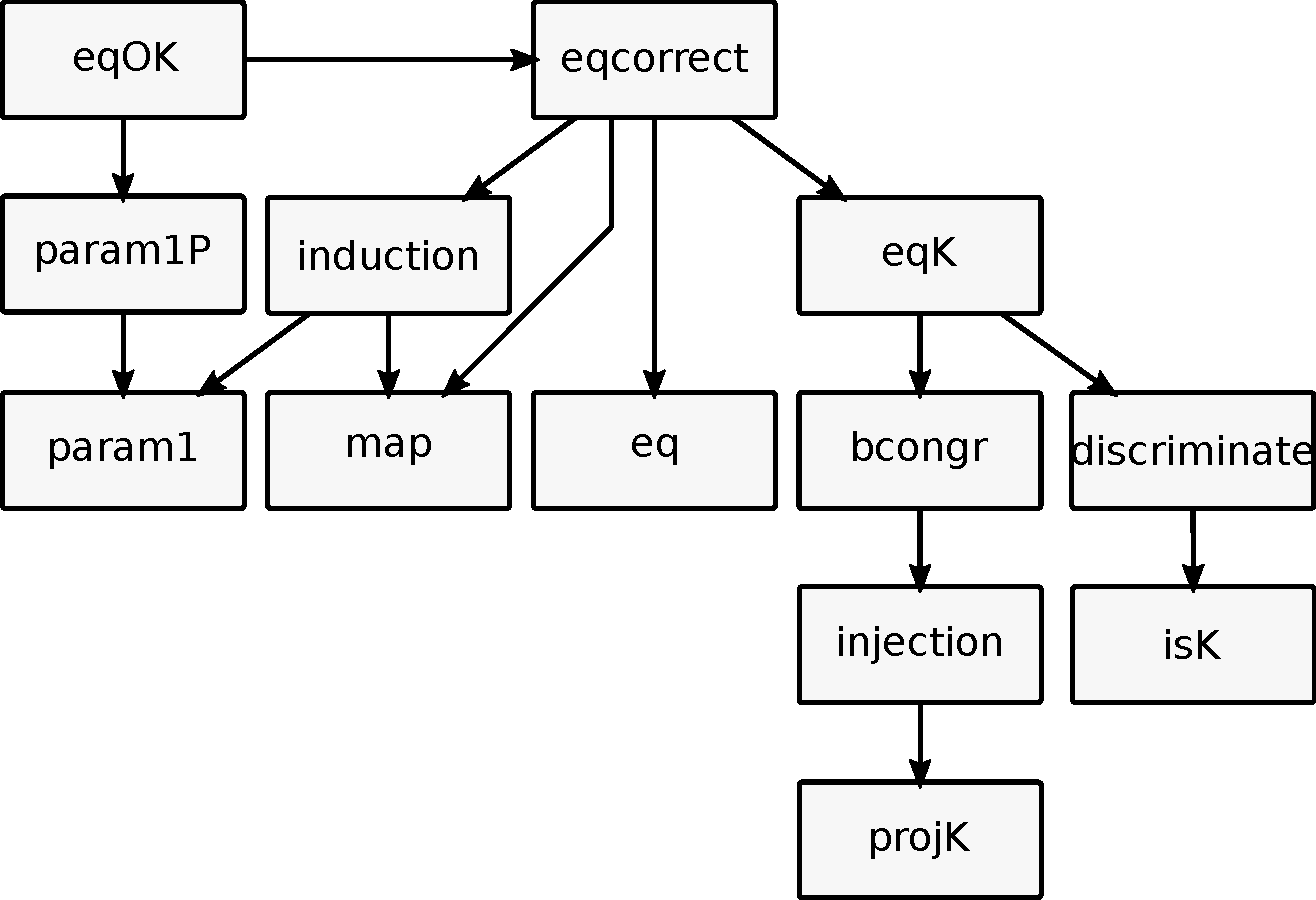
\includegraphics[width=0.45\textwidth]{derive.pdf}

The \derive{eq} component is in charge on synthesizing the program
performing the equality test. Recursion is performed on the first
term; then the two terms are inspected via pattern matching. If the
constructors are different the output is false, otherwise the
results of the recursive calls on the subterms are composed using
boolean conjunction.

The correctness proof generated by \derive{eqcorrect} goes by induction on
the first term of the two being compared and then the proof goes on
in a different branch for each constructor K. 
The property being proved by induction is expressed
using \lstinline+eq_axiom+ that, as we will detail in
section~\ref{sec:reflect} is equivalent to a double implication.
The \derive{bcongr} component proves that the property is preserved
by equal contexts, that is when the two terms are built using the
same constructor. When they are not the program must return false
and the equality be false as well: this is shown by \derive{eqK},
that performs the case split on the second term. The no confusion
property of constructor is key to this contextual reasoning.
\derive{projK} and \derive{isK} generate utility functions that
are then used by \derive{injection} and \derive{discriminate} to
prove that constructors are injective and different.
As we sketched in the previous sections the unary parametricity
translation plays a key role in expressing the induction
principle. The inductive predicate \lstinline+is_T+ for an inductive
type \lstinline+T+ is generated by \derive{param1} while
\derive{param1P} shows that terms of type \lstinline+T+ validate
\lstinline+is_T+. \derive{map} shows that \lstinline+is_T+ is a
functor when \lstinline+T+ has parameters. This property is both
used to synthesize induction principles and also to combine the
pieces together in the correctness proof.
The \derive{eqOK} component hides the \lstinline+is_T+ relation
from the theorems proved by \derive{eqcorrect} by using the lemmas
proved by \derive{param1P}.

\subsection{Equality test} %%%%%%%%%%%%%%%%%%%%%%%%%%%%%%%%%%%%%%%%%%%%%%%%%%%%%%%%%%

Synthesizing the equality test for a type \lstinline+T+ is the
simplest step.  For each type parameter \lstinline+a+ an equality test
\lstinline+a_eq+ has to be taken in input.  Then the recursive function
takes in input two terms of type \lstinline+T+ and inspects both via
pattern matching.  Outside the diagonal, where constructors are
different, we return \lstinline+false+. On the diagonal we compose the
calls on the arguments of the constructors using boolean conjunction.
The code called to compare two arguments depend on their type. If it
is \lstinline+T+ then it is a recursive call. If it is a type
parameter \lstinline+a+ then we use \lstinline+a_eq+. If it is
another type constructor we use the equality test for it.

Lets take for example the equality test for rose trees:

\begin{minipage}{\textwidth}\begin{lstlisting}[numbers=left]
Definition |+rtree_eq+| A (A_eq : A -> A -> bool) :=
  fix rec (t1 t2 : rtree A) {struct t1} : bool :=
  match t1, t2 with
  | Leaf a, Leaf b  => A_eq a b
  | Node l, Node s => list_eq (rtree A) rec l s
  | _, _ => false
  end.
\end{lstlisting}\end{minipage}

\noindent
Line 5 calls \lstinline+list_eq+ since the type of \lstinline+l+ and
\lstinline+s+ is \lstinline+(list (rtree A))+ and it passes to it
\lstinline+rec+ since the type parameter of \lstinline+list+ is
\lstinline+(rtree A)+.

Elpi is a logic programming language: programs are organized in
clauses that represent both a data base of known facts
and a set of rules to derive new facts out of known ones.
In this particular case we use the \lstinline+eq-db+ relation
to link a type to its equality test. Here an excerpt of Elpi
code.\footnote{We deliberately simplify the syntax of Elpi 
since the omitted details are not relevant for this paper.
For example \lstinline+list_eq+, being a definition,
is actually written \lstinline+(const "Coq.Demo.list_eq")+; 
\lstinline+list+, being an inductive type,
is written \lstinline+(indt "Coq.Init.Datatypes.list")+;
\lstinline+A+, being a bound variable, is represented by
a unique nominal constant \lstinline+c0+.}

\begin{minipage}{\textwidth}\begin{lstlisting}[numbers=left]
eq-db "A" "A_eq".
eq-db (app["rtree","A"]) "aux".
eq-db (app["list", B]) (app["list_eq", B, B_eq]) :-
  eq-db B B_eq.
\end{lstlisting}\end{minipage}

\noindent
Elpi represent Coq terms in HOAS style,
hence the application node \lstinline+app+ becomes apparent.
Also, following the syntactic
convention of Prolog, capital letters are variables.
Note that \lstinline+"A"+ is a fixed Coq term,
in this case the first argument of \lstinline+rtree_eq+, while
\lstinline+B+ is an Elpi variable, that is a parameter
of the clause.

The first two clauses are facts, respectively stating that
\lstinline+A_eq+ is the equality test for type
\lstinline+A+, and that \lstinline+aux+ is the one for
\lstinline+(rtree A)+. 
The third clause is an inference one and reads: the equality test
for \lstinline+(list B)+ is \lstinline+(list_eq B B_eq)+ \emph{if}
\lstinline+B_eq+ is the one for \lstinline+B+.

Finally note that the first two clauses are present only during the
derivation. Once it is complete they are both removed and the
following one is permanently added to the data base.

\begin{minipage}{\textwidth}\begin{lstlisting}[]
eq-db (app["rtree", B]) (app["rtree_eq", B, B_eq]) :-
  eq-db B_eq.
\end{lstlisting}\end{minipage}


% This derivation covers polynomial types and simple indexed data types
% such as vectors. When indexes are present the fixpoint decorrelates
% the index value of the two terms, e.g.:
% 
% \begin{minipage}{\textwidth}\begin{lstlisting}
% Definition vector_eq a i (v1 v2 : vector a i) :=
%   fix rec i (v1 : vector a i) j (v2 : vector a j) :=
%     .. nat_eq pi pj && rec pi xs pj ys ..
%   in
%     rec i v1 i v2
% \end{lstlisting}\end{minipage}
% 
% \noindent
% In this way \lstinline{rec} can be applied to sub vectors
% \lstinline{xs} and \lstinline{ys} without having to prove,
% on the spot, that their lengths \lstinline+pi+ and \lstinline+pj+
% are equal.

\subsection{Parametricity} %%%%%%%%%%%%%%%%%%%%%%%%%%%%%%%%%%%%%%%%%%%

The \derive{pram1} component is able to generate the unary
parametricity translation of types and terms
following~\cite{keller:hal-00730913}. We already gave a few
examples in section~\ref{sec:idea}, we repeat here just the
one for rose trees:

\begin{minipage}{\textwidth}\begin{lstlisting}
Inductive is_rtree A (PA: A -> U): rtree A -> U :=
| is_Leaf a (pa : PA a) : is_rtree A PA (Leaf A a)
| is_Node l (pl : is_list (rtree A) (is_rtree A PA) l) :
    is_rtree A PA (Node A l).
\end{lstlisting}\end{minipage}

\noindent
The \derive{pram1P} component synthesizes proofs that terms
of type \lstinline+T+ validate \lstinline+is_T+.
In section~\ref{sec:idea:transparent} we explained why
these proofs needs to be transparent.

\begin{minipage}{\textwidth}\begin{lstlisting}
Definition |+rtree_is_rtree+| A (PA : A -> U) :
  (forall x, PA x) -> forall t, is_rtree A PA t.
\end{lstlisting}\end{minipage}

\noindent
It is worth pointing out that the premise
\lstinline+(forall x, PA x)+ can be proved not only for
trivial \lstinline+PA+. In particular, during induction
on a term of type \lstinline+T+ the predicate being
proved, say \lstinline+P+, is true by induction hypothesis
on (smaller) terms of type \lstinline+T+. See for example
line 10 in the proof of \lstinline+rtree_eq_correct+ in
section~\ref{sec:idea:transparent}.


\subsection{Functoriality} %%%%%%%%%%%%%%%%%%%%%%%%%%%%%%%%%%%%%%%%%%%%%%%%%%%%%%%%%%%

The \derive{map} components implements a double service.

For simple containers it synthesizes what one expects. For example:

\begin{minipage}{\textwidth}\begin{lstlisting}
Definition rtree_map A1 A2 :
  (A1 -> A2) -> rtree A1 -> rtree A2.
\end{lstlisting}\end{minipage}

The derivation on containers with no indexes is not needed in order
to synthesize equality tests nor their correctness proofs.
On the contrary it becomes crucial when the container has indexes,
e.g. when the container is a \lstinline+is_T+ inductive predicate.

On indexed data types the derivation avoids to map the indexes and
consequently all type variables occurring in the types of the indexes.
For example, mapping the \lstinline+is_list+ inductive predicate gives:

\begin{minipage}{\textwidth}\begin{lstlisting}
Lemma is_list_map : A PA PB,
  (forall a, PA a -> PB a) ->
    forall l, is_list A PA l -> is_list A PB l.
\end{lstlisting}\end{minipage}

\noindent
This property corresponds to the functoriality of \lstinline+is_list+
over the property about the type parameter. 

Since Elpi is a logic programming language we can express
these maps as clauses and use the data base later on in the
\derive{induction} and \derive{eqcorrect} derivations.
Here an excerpt:

\begin{minipage}{\textwidth}\begin{lstlisting}[]
map-db (app["is_list", A, PA])
        (app["is_list", A, PB]) R :-
  R = (app["is_list_map", A, PA, PB, F]),
  map-db PA PB F.
\end{lstlisting}\end{minipage}

\noindent
Note that the terms are ``point free'', i.e.
the first two arguments are terms of arity one, while
the third term is of arity two. For example the identity
map would be written as follows:

\begin{minipage}{\textwidth}\begin{lstlisting}[]
map-db PA PA (lam (fun a pa => pa)).
\end{lstlisting}\end{minipage}



\subsection{Induction} %%%%%%%%%%%%%%%%%%%%%%%%%%%%%%%%%%%%%%%%%%%%%%%%%%%%%%
\label{sec:induction}

In order to derive the induction principle for type
\lstinline+T+ we first derive its unary parametricity
translation \lstinline+is_T+. 

The \lstinline+is_T+ inductive
predicate has one constructor \lstinline+is_K+ for each
constructor \lstinline+K+ of the type \lstinline+T+.
The type of \lstinline+is_K+ relates to the type of
\lstinline+K+ in the following way. For each
argument \lstinline+(a : A)+
of \lstinline+K+, \lstinline+is_K+ takes two arguments:
\lstinline+(a : A)+ and \lstinline+(pa : is_A a)+.
Finally the type of \lstinline+is_K a1 pa1 .. an pan+ is
\lstinline+is_T (K a1 .. an)+.

The induction principle can be synthesized as follows:
\begin{enumerate}
\item take in input each parameter
  \lstinline+A1 PA1 .. An PAn+ of \lstinline+is_T+
\item take in input a predicate \lstinline+(P : T A1 .. An -> U)+
\item for each constructor \lstinline+(is_K : S)+ 
  take an assumption \lstinline+HK+ of type
  \lstinline+S[is_T A1 PA1 .. An PAn / P]+
  (\lstinline+S+ where \lstinline+is_T |*A*|+ is replaced by
  \lstinline+P+)
\item take in input \lstinline+(t : T A1 .. An)+ and
  \lstinline+(x : is_T A1 PA1 .. An PAn)+.
\item recursion is performed on \lstinline+x+
\item each branch binds the arguments of constructor \lstinline+is_K+
  as \lstinline+(a1 : A1) (pa1 : is_A1 a1) .. (an : An) (pan : is_An an)+
  and returns \lstinline+HK a1 qa1 .. an qan+ where
  \lstinline+qai+ is obtained by \emph{mapping} the corresponding
  \lstinline+pai+ (as in \lstinline+map-db+).
\end{enumerate}

Lets take for example the induction principle for rose trees:

\begin{minipage}{\textwidth}\begin{lstlisting}
Definition rtree_induction A PA P  
    (HLeaf : forall a, PA a -> P (Leaf A a))
    (HNode : forall l, is_list (rtree A) P l -> P (Node A l)) :
  forall t, is_rtree A PA t -> P t
:=
  fix IH (t : rtree A) (x : is_rtree A PA t) {struct x} : P t :=
  match x with
  | is_Leaf a pa => HLeaf a pa
  | is_Node l pl => (* pl : is_list (rtree A) (is_rtree A PA) l *)
      HNode l
        (is_list_map (rtree A) (is_rtree A PA) P IH l pl)
  end.
\end{lstlisting}\end{minipage}

Note how the type of \lstinline+HLeaf+ can be obtained fom the
type of \lstinline+is_Leaf+ by replacing \lstinline+(is_rtree A PA)+
with \lstinline+P+.

Finally lets see  how the second argument to \lstinline+HNode+ is
synthesized.  We take advantage of the fact that Elpi is a logic
programming language and we query the data base \lstinline+map-db+
as follows. First we temporarily register 
the fact that \lstinline+IH+ maps
\lstinline+(is_rtree A PA)+ to \lstinline+P+ obtaining, among others,
the following clauses.

\begin{minipage}{\textwidth}\begin{lstlisting}[]
map-db (app["is_rtree", "A", "PA"]) "P" "IH".
map-db (app["is_list", A, PA])
        (app["is_list", A, PB]) R :-
  R = (app["is_list_map", A, PA, PB, F]),
  map-db PA PB F.
\end{lstlisting}\end{minipage}

Then we query \lstinline+map-db+ as follows:

\begin{minipage}{\textwidth}\begin{lstlisting}[]
map-db (app["is_list", app["rtree","A"],
           app["is_rtree","A","PA"]])
        (app["is_list", app["rtree","A"],
           "P"]) Q.
\end{lstlisting}\end{minipage}

\noindent
The answer

\begin{minipage}{\textwidth}\begin{lstlisting}[]
Q = app["is_list_map", app["rtree","A"],
         app["is_rtree","A","PA"], "P",
         "IH"]
\end{lstlisting}\end{minipage}

\noindent
is exactly the second term we need to pass to \lstinline+HNode+
(once applied to \lstinline+l+ and \lstinline+Pl+).

To sum up the unary parametricity translation give us the type
of the induction principle, up to a trivial substitution.
The functoriality property of the inductive predicates obtained by
parametricity gives us a way to prove the branches.

\subsection{No confusion property} %%%%%%%%%%%%%%%%%%%%%%%%%%%%%%%%%%%%%%%%%%%%

In order to prove that an equality test is correct
one has to show the ``no confusion'' property, that is that
constructors are injective and disjoint.

Lets start by provide they are disjoint.
The simples form of this property can be expressed on bool:

\begin{minipage}{\textwidth}\begin{lstlisting}
Lemma |+bool_discr+| : true = false -> forall T : U, T.
\end{lstlisting}\end{minipage}

\noindent
This lemma is proved by hand once and forall. What the \derive{isK}
component synthesizes is a per-constructor test to be used in order
to reduce a discrimination problem on type \lstinline+T+ to a
discrimination problem on \lstinline+bool+. For the rose tree data
type \derive{isK} generates the following consants:

\begin{minipage}{\textwidth}\begin{lstlisting}
Definition rtree_is_Node A (t : rtree A) : bool :=
  match t with Node _ => true | _ => false end.
Definition rtree_is_Leaf A (t : rtree A) : bool :=
  match t with Node _ => false | _ => true end.
\end{lstlisting}\end{minipage}

\noindent
The \derive{discriminate} components uses one more trivial fact,
\lstinline+eq_f+ in order to assemble these tests together
with \lstinline+bool_discr+.

\begin{minipage}{\textwidth}\begin{lstlisting}
Lemma |+eq_f+| T1 T2 (f : T1 -> T2) :
  forall a b, a = b -> f a = f b.
\end{lstlisting}\end{minipage}

\noindent
From a term \lstinline+H+ of type 
\lstinline+(Node l = Leaf a)+ the \derive{discriminate} procedure
synthesizes a term of type \lstinline+(forall T : U, T)+ as follows:

\begin{minipage}{\textwidth}\begin{lstlisting}[numbers=left]
bool_discr
  (eq_f (rtree A) (rtree A) (rtree_is_Node A) H)
\end{lstlisting}\end{minipage}

\noindent
Note that the type of the term on line 2 is:

\begin{minipage}{\textwidth}\begin{lstlisting}
  rtree_is_Node A (Node l) = rtree_is_Node A (Leaf a)
\end{lstlisting}\end{minipage}

\noindent
that is convertible to \lstinline+(true = false)+.

In order to prove the injectivity on constructors the \derive{projK}
produce synthesizes a projector for each argument of each constructor.
For example

\begin{minipage}{\textwidth}\begin{lstlisting}
Definition list_get_cons1 A (d1 : A) (d2 : list A)
  (l : list A) : A
:=
  match l with
  | nil => d1
  | cons x _ => x
  end.

Definition list_get_cons2 A (d1 : A) (d2 : list A)
  (l : list A) : list A
:=
  match l with
  | nil => d2
  | cons _ xs => xs
  end.
\end{lstlisting}\end{minipage}

\noindent
Each projector takes in input default values for each and every
argument of the constructor. It is designed to be used by the
\derive{injection} procedure as follows. Given a term
\lstinline+H+ of type \lstinline+(cons x xs = cons y ys)+, in order
to obtain a term of type \lstinline+(xs = ys)+ it generates:

\begin{minipage}{\textwidth}\begin{lstlisting}[numbers=left]
eqf H (list_get_cons2 A x xs)
\end{lstlisting}\end{minipage}

\noindent
This term is easy to build given the type of \lstinline+H+ that
contains the default values to be passed to the projector.
Note that the type of the entire term is:

\begin{minipage}{\textwidth}\begin{lstlisting}
list_get_cons2 A x xs (cons x xs) =
  list_get_cons2 A x xs (cons y ys)
\end{lstlisting}\end{minipage}

\noindent
that is convertible to the desired \lstinline+(xs = ys)+.

\subsection{Congruence and \lstinline+reflect+} %%%%%%%%%%%%%%%%%%%%%%%%%%%%%%%%%%%%%%%%%%%%%%%%%%%%%%%
\label{sec:reflect}

In the definition of \lstinline+eq_axiom+ we used the \lstinline+reflect+
predicate. It is a form of if-and-only-if specialized to link a
proposition and a boolean test. It is defined as follows:

\begin{minipage}{\textwidth}\begin{lstlisting}
Inductive reflect (P : U) : bool -> U :=
| ReflectT (p : P) : reflect P true
| ReflectF (np : P -> False) : reflect P false.
\end{lstlisting}\end{minipage}

\noindent
To prove the correctness of equality tests the shape of
\lstinline+P+ is always an equation between two terms of
the inductive type, most of the time constructors.
When it find the same constructor on both sides, as in
\lstinline+(k x1 .. xn = k y1 .. y2)+, the equality tests
calls appropriate equality tests for the arguments and forgets about
the constructor. The \derive{bcongr} component synthesizes lemmas
helping this step. For example:

\begin{minipage}{\textwidth}\begin{lstlisting}
Lemma list_bcongr_cons A :
    forall (x y : A) b, reflect (x = y) b ->
    forall (xs ys : list A) c, reflect (xs = ys) c ->
  reflect (x :: xs = y :: ys) (b && c)

Lemma rtree_bcongr_Leaf A (x y : A) b :
  reflect (x = y) b -> reflect (Leaf A x = Leaf A y) b

Lemma rtree_bcongr_Node A (l1 l2 : list (rtree A)) b :
  reflect (l1 = l2) b -> reflect (Node A l1 = Node A l2) b
\end{lstlisting}\end{minipage}

\noindent
Note that these lemmas are not related to the
equality test specific to the inductive type. Indeed they deal
with the \lstinline+reflect+ predicate, but not with the
\lstinline+eq_axiom+ that we use every time we talk about equality tests.

The derivation goes as follows: if any of the premises about
\lstinline+reflect+ is false, then the result is probed by
\lstinline+ReflectF+ and the injectivity of constructors.
If all premises are \lstinline+ReflectT+ their argument,
an equation, can be used to rewrite the conclusion.

\begin{minipage}{\textwidth}\begin{lstlisting}
Lemma list_bcongr_cons A :
    forall (x y : A) b, reflect (x = y) b ->
    forall (xs ys : list A) c, reflect (xs = ys) c ->
  reflect (x :: xs = y :: ys) (b && c)
:=
  fun x y b (hb : reflect (x = y) b)
      xs ys c (hc : reflect (xs = ys) c) =>
  match hb, hc with
  | ReflectT eq_refl, ReflectT eq_refl => ReflectT eq_refl
  | ReflectF (e : x = y -> False), _ =>
    ReflectF
      (fun H : (x :: xs) = (y :: ys) =>
       e (eq_f (list A) A (list_get_cons1 A x xs)
         (x :: xs) (y :: ys) H))
  | _, ReflectF e => ..injection..
end.
\end{lstlisting}\end{minipage}

This is a sort of injection but specialized to Ks, to avoid n-ary
injection.

This step corresponds to rec call + propagate return value.

\subsection{Congruence and \lstinline+eq_axiom+} %%%%%%%%%%%%%%%%%%%%%%%%%%%%%%%%%%%%%%%%%%%%%%%%

Now discrimination, the real switch, eg 2 different constructors.
generate false in one case, call bcongr in the other.

\begin{minipage}{\textwidth}\begin{lstlisting}
Lemma rtree_eq_axiom_Node A (f : A -> A -> bool) l1 :
    eq_axiom (list (rtree A)) (list_eq (rtree A) (rtree_eq A f)) l1 ->
  eq_axiom (rtree A) (rtree_eq A f) (Node A l1)
:=
  fun h (t2 : rtree A) =>
  match t2 with
  | Leaf n =>
    ReflectF (fun abs : Node A l1 = Leaf A n =>
      bool_discr
        (eq_f (rtree A) bool (rtree_is_Node A)
	  (Node A l1) (Leaf A n) abs)
        False)
  | Node l2 =>
      rtree_bcongr_Node A l1 l2
        (list_eq (rtree A) (rtree_eq A f) l1 l2) (h l2)
end.
\end{lstlisting}\end{minipage}

\subsection{Correctness} %%%%%%%%%%%%%%%%%%%%%%%%%%%%%%%%%%%%%%%%%%%%%%%%
\label{sec:derive:eqcorrect}

The \derive{eqcorrect} component combines the induction
principle generated by \derive{induction} with the
case split on the second term provided by \derive{eqK}.

Lets recall the type of the correctness lemma for
\lstinline+list_eq+, of the induction principle
and then analyze the proof of
\lstinline+rtree_eq_correct+:

\begin{minipage}{\textwidth}\begin{lstlisting}
Lemma |+list_eq_correct+| A (fa : A -> A -> bool) l,
    is_list A (eq_axiom A fa) l ->
  eq_axiom (list A) (list_eq A fa) l.

Definition rtree_induction A PA P  
    (HLeaf : forall y, PA y -> P (Leaf A y))
    (HNode : forall l, is_list (rtree A) P l -> P (Node A l)) :
  forall t, is_rtree A PA t -> P t.

Lemma rtree_eq_axiom_Node A (f : A -> A -> bool) l1 :
    eq_axiom (list (rtree A)) (list_eq (rtree A) (rtree_eq A f)) l1 ->
  eq_axiom (rtree A) (rtree_eq A f) (Node A l1).
       
Lemma |+rtree_eq_correct+| A (fa : A -> A -> bool) :=
  rtree_induction A (eq_axiom A fa)
(*P*)     (eq_axiom (rtree A) (rtree_eq A fa))
(*HLeaf*) (rtree_eq_axiom_Leaf A fa)
(*HNode*) (fun l (Pl : is_list (rtree a)
                   (eq_axiom (rtree a) (rtree_eq a fa)) l) =>
             rtree_eq_axiom_Node A fa l
               (list_eq_correct (rtree a) (rtree_eq a fa) l Pl)).
\end{lstlisting}\end{minipage}

Logic programming provides again a natural way to guide the
derivation. In particular we use the \lstinline+map-db+ predicate
to link the hypotheses provided by the induction principle,
such as \lstinline+Pl+, to the premises of the branch lemmas
produced by \derive{eqK}. 

\begin{minipage}{\textwidth}\begin{lstlisting}[]
map-db (is_list A PA)
       (eq_axiom (list A) (list_eq A F))
       (list_eq_correct A F) :- map-db PA (eq_axiom A F).
       FIXME
\end{lstlisting}\end{minipage}

\noindent
We extend the \lstinline+map-db+ predicate, instead of building
a new one just for correctness lemmas, because functoriality lemmas
are sometimes needed. Take for example this simple data type
of an histogram.

\begin{minipage}{\textwidth}\begin{lstlisting}[numbers=left]
Inductive histogram := Columns (bars : list nat).

Lemma histogram_induction (P : histogram -> Type) :
    (forall l, is_list nat is_nat l -> P (Columns l)) ->
  forall h, is_histogram h -> P h.

Lemma histogram_eq_axiom_Columns :
    forall l : list nat, eq_axiom (list nat) (list_eq nat nat_eq) l ->
  forall h, eq_axiom_at histogram histogram_eq (Columns l) h.

Lemma histogram_eq_correct 
  forall (h : histogram), eq_axiom (histogram A) (histogram_eq A fa) h
:=
  histogram_induction 
    (eq_axiom histogram histogram_eq)
    (fun l (Pl : is_list nat is_nat l) =>
       histogram_eq_axiom_Columns
         l (list_eq_correct nat nat_eq
              l (is_list_map nat
                   is_nat (eq_axiom nat nat_eq)
                   nat_eq_correct l Pl))).
\end{lstlisting}\end{minipage}

\noindent
Note that Pl's type \lstinline+is_list nat is_nat+
needs to be mapped to \lstinline+is_list nat (eq_axiom nat nat_eq)+,
hence \lstinline+nat_eq_correct+ cannot be used directly
but must undergo the \lstinline+is_list+ functor.

\subsection{eqOK} %%%%%%%%%%%%%%%%%%%%%%%%%%%%%%%%%%%%%%%%%%%%%%%%%%%%%

The last derivation hides the \lstinline+is_T+ to the final user.

\begin{minipage}{\textwidth}\begin{lstlisting}
Lemma |+list_eq_correct+| A fa :
  forall l, is_list A (eq_axiom A  fa) l ->
    eq_axiom list A (list_eq A  fa) l.

Lemma |+list_eq_OK+| A f (Hf : forall a, eq_axiom A f a) :
  eq_axiom list A (list_eq A f)
:=
  fun l => list_eq_correct A f (list_is_list A Hf) l.
\end{lstlisting}\end{minipage}


%%%%%%%%%%%%%%%%%%%%%%%%%%%%%%%%%%%%%%%%%%%%%%%%%%%%%%%%%%%%%%%%%%%%%%%%%%%
\section{Implementation} %%%%%%%%%%%%%%%%%%%%%%%%%%%%%%%%%%%%%%%%%%%%%%%%%%
\label{sec:elpi}

As we sketched in section~\ref{sec:code} the derivations are
implemented using the Elpi extension language for Coq.

Elpi is a logic programming language based on $\lambda$Prolog.
Object language terms are described using the Higher Order Abstract
Syntax approach, that mean the programmer needs not to care about the
representation of bound variables. The other features of Elpi
are not relevant for this paper.

The Coq-elpi plugin for Coq implements the HOAS encoding of Coq
terms and provides way to register commands such as
\lstinline+Elpi derive+ and provides a few API to access the
logical environment of Coq, that is to read and declare
types and to read and define terms.

The code quite compact, thanks to the fact that the programming
language is very high level and its programming paradigm is a good
for for this application.

\begin{tabular}{ll}
   96 & derive/bcongr.elpi\\
   71 & derive/derive.elpi\\
  162 & derive/eq.elpi\\
   82 & derive/eqK.elpi\\
  104 & derive/eqOK.elpi\\
  117 & derive/induction.elpi\\
   34 & derive/isK.elpi\\
  214 & derive/map.elpi\\
  200 & derive/param1.elpi\\
   85 & derive/param1P.elpi\\
  126 & derive/projK.elpi\\
   73 & derive/tysimpl.elpi\\
   87 & engine/reduction.elpi\\
  314 & coq-HOAS.elpi \\
  344 & coq-builtin.elpi
\end{tabular}

\subsection{Incompleteness and user intervention} %%%%%%%%%%%%%%%%%%%%%%%%%
\label{sec:oops}

At the time of writing Coq-elpi does not support mutual inductive
types, universe polymorphic definitions and primitive projections.

The code supports polynomial types. Some derivations do
support index data, eg \derive{eq} is able to synthesize
an equality test for vectors. Most of the derivations about
contextual reasoning, such as \derive{eqK} and \derive{bcongr}
do not support indexes. A was to do that for indexes that admit a
decidable equality is to wrap. For example \derive{projK} derives
this

\begin{minipage}{\textwidth}\begin{lstlisting}
projcons3
     : forall (A : Type) (H : nat),
       A ->
       forall n : nat,
       Vector.t A n -> Vector.t A H -> {i1 : nat & Vector.t A i1}
\end{lstlisting}\end{minipage}

\noindent
For this you need an eqType, that is what we derive in this work,
hence supporting more is future work. We did it by hand, 20 lines of
boilerplate linking regular and wrapped vectors, and 20 lines proving
by hand what \derive{eqK} abd \derive{bcongr} could do.

performance wise...

%%%%%%%%%%%%%%%%%%%%%%%%%%%%%%%%%%%%%%%%%%%%%%%%%%%%%%%%%%%%%%%%%%%%%%%%%%
\section{Related work} %%%%%%%%%%%%%%%%%%%%%%%%%%%%%%%%%%%%%%%%%%%%%%%%%%%
\label{sec:related}

Systems similar to Coq, eg Matita, Lean, Agda and Isabelle all generate
induction principles automatically, and some of them also the
no confusion properties. To our knowledge they do not generate
sensible induction principles when containers are involved.

Coq provides two mechanisms related to this work.
Scheme equality bla bla does not support containers.
The decide equality tactic is not fully automatic,
mixes the computational code with the proof by using sigT
and finally inlines things.

In the programming language world derivation is much more developed.
The dominant approach is to provide some meta programming facilities,
eg by providing a syntactic declaration of types and the use the
programming language itself to write derivations. Our approach
is similar in a sense, we work at the meta level on the syntax of
types, but very different since we, on purpose, pick a different
language for meta programming. We pick a high level one that makes
our derivations very concise and hides uninteresting details such
as bound variables.

%%%%%%%%%%%%%%%%%%%%%%%%%%%%%%%%%%%%%%%%%%%%%%%%%%%%%%%%%%%%%%%%%%%%%%%%%%%
\section{Conclusion} %%%%%%%%%%%%%%%%%%%%%%%%%%%%%%%%%%%%%%%%%%%%%%%%%%%%%%
\label{sec:conclusion}

We described a technique to define better induction principles
for Coq data types built using containers. We used the unary
parametricity translation in order to separate terms from types,
express structural properties and finally confine the modularity
problems stemming from the termination check implemented in Coq.
Finally we provide a Coq package deriving correct equality tests
for polynomial inductive data types.

It seems reasonable to extend the current derivation code to cover
inductive types with decidable indexes, as hinted in
section~\ref{sec:oops}. For types not covered, it should be possible
to improve the way user intervention is requested: right now errors
are printed, but the exact type of the missing lemma has to be written
down by the user.
Finally, we look forward to let the user tune
the derivation process by annotating the type declaration, eg to skip
certain arguments when generating the equality test, for example the
integer describing the length of a sub vector. The resulting equality
test will surely require some user intervention to be proved correct,
but will be better behaved wrt extraction.

\begin{acks}
We thank Maxime Denes and Cyril Cohen for many discussions shedding light
on the subject; Cyril Cohen for the code implementing the parametricity
translation in Elpi; Luc Chabassier for working on an early prototype of
Elpi on the synthesis of equality tests, an experiment that convinced
the author it was actually doable.
\end{acks}


%% Bibliography
\bibliography{bibfile}


%% Appendix
\appendix
\section{Appendix}

Text of appendix \ldots

\end{document}
% vim set: textwidth=70:
